% This file was created with tikzplotlib v0.10.1.
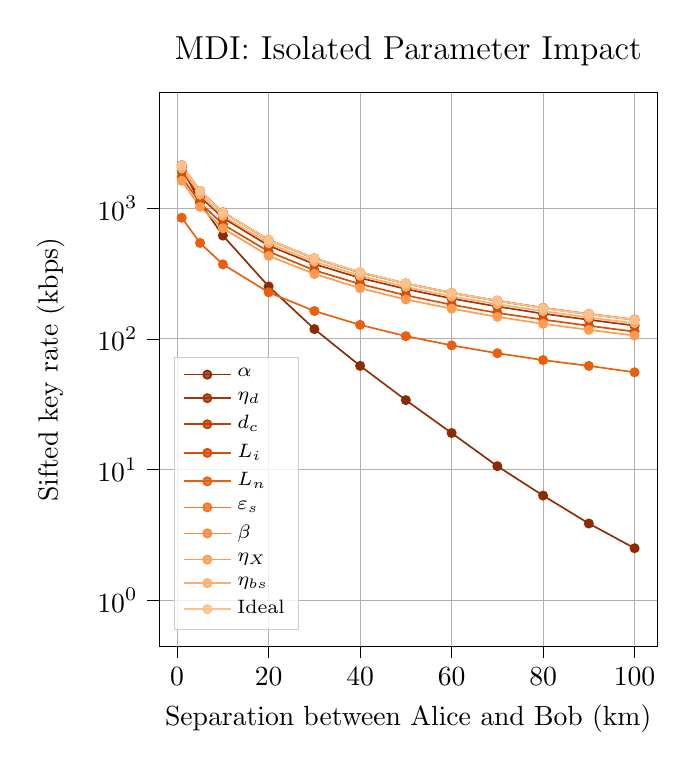
\begin{tikzpicture}

\definecolor{burlywood253194140}{RGB}{253,194,140}
\definecolor{chocolate2339513}{RGB}{233,95,13}
\definecolor{chocolate24411531}{RGB}{244,115,31}
\definecolor{coral25113554}{RGB}{251,135,54}
\definecolor{darkgray176}{RGB}{176,176,176}
\definecolor{firebrick193631}{RGB}{193,63,1}
\definecolor{lightgray204}{RGB}{204,204,204}
\definecolor{orangered220763}{RGB}{220,76,3}
\definecolor{saddlebrown141443}{RGB}{141,44,3}
\definecolor{saddlebrown164533}{RGB}{164,53,3}
\definecolor{sandybrown25315681}{RGB}{253,156,81}
\definecolor{sandybrown253174108}{RGB}{253,174,108}

\begin{axis}[
width=180pt,
height=200pt,
scale only axis,
legend cell align={left},
legend style={
  fill opacity=0.8,
  draw opacity=1,
  text opacity=1,
  at={(0.03,0.03)},
  anchor=south west,
  draw=lightgray204,
  font=\fontsize{7}{9}\selectfont
},
log basis y={10},
tick align=outside,
xtick pos=left,
ytick pos=left,
tick label style={font=\fontsize{10}{12}\selectfont},
label style={font=\fontsize{10}{12}\selectfont},
title style={font=\fontsize{12}{14}\selectfont},
title={MDI: Isolated Parameter Impact},
x grid style={darkgray176},
xlabel={Separation between Alice and Bob (km)},
xmajorgrids,
xmin=-3.95, xmax=104.95,
xtick style={color=black},
xtick={-20,0,20,40,60,80,100,120},
xticklabels={
  \(\displaystyle {\ensuremath{-}20}\),
  \(\displaystyle {0}\),
  \(\displaystyle {20}\),
  \(\displaystyle {40}\),
  \(\displaystyle {60}\),
  \(\displaystyle {80}\),
  \(\displaystyle {100}\),
  \(\displaystyle {120}\)
},
y grid style={darkgray176},
ylabel={Sifted key rate (kbps)},
ylabel style={yshift=5pt},
ymajorgrids,
ymin=0.443301364171667, ymax=7669.68788693672,
ymode=log,
ytick style={color=black},
ytick={0.01,0.1,1,10,100,1000,10000,100000},
yticklabels={
  \(\displaystyle {10^{-2}}\),
  \(\displaystyle {10^{-1}}\),
  \(\displaystyle {10^{0}}\),
  \(\displaystyle {10^{1}}\),
  \(\displaystyle {10^{2}}\),
  \(\displaystyle {10^{3}}\),
  \(\displaystyle {10^{4}}\),
  \(\displaystyle {10^{5}}\)
}
]
\addplot [semithick, saddlebrown141443, mark=*, mark size=1.5, mark options={solid}]
table {%
1 2054.2244670438
5 1107.78813481042
10 618.788503345538
20 252.30168132166
30 119.015569905839
40 62.2126121610172
50 33.9867668138561
60 19.0408669002778
70 10.6076825411772
80 6.31738266900979
90 3.86319988397186
100 2.49738859917583
};
\addlegendentry{$\alpha$}
\addplot [semithick, saddlebrown164533, mark=*, mark size=1.5, mark options={solid}]
table {%
1 1941.92978729554
5 1229.39330624988
10 845.987336656331
20 517.991542283896
30 373.985348598467
40 292.931347322571
50 241.150439771231
60 203.787182444142
70 177.161902573774
80 156.156216223152
90 140.145143947873
100 126.606634521768
};
\addlegendentry{$\eta_d$}
\addplot [semithick, firebrick193631, mark=*, mark size=1.5, mark options={solid}]
table {%
1 2135.53859991693
5 1355.48107164318
10 932.347157357019
20 574.827545979573
30 414.737191630501
40 323.374046306424
50 265.324803413977
60 225.280854516648
70 196.26669214975
80 172.754775707697
90 154.607699418209
100 140.784227457337
};
\addlegendentry{$d_c$}
\addplot [semithick, orangered220763, mark=*, mark size=1.5, mark options={solid}]
table {%
1 1726.99836846101
5 1104.63385403785
10 753.838861756156
20 466.923356608342
30 335.559401104289
40 263.222199041698
50 215.685047674337
60 182.884463654718
70 158.171834551427
80 140.683335034701
90 126.222716472423
100 113.664345946907
};
\addlegendentry{$L_i$}
\addplot [semithick, chocolate2339513, mark=*, mark size=1.5, mark options={solid}]
table {%
1 847.292559563737
5 543.355129100678
10 372.535321357348
20 227.37666114566
30 163.662269321357
40 128.148922843449
50 105.051645490385
60 89.2664044757766
70 77.7320871432128
80 68.8601831057747
90 62.1740733472798
100 55.5773877619856
};
\addlegendentry{$L_n$}
\addplot [semithick, chocolate24411531, mark=*, mark size=1.5, mark options={solid}]
table {%
1 2140.57299790117
5 1360.38906818831
10 932.301923522926
20 568.926373358709
30 413.174876415507
40 322.077589246902
50 266.227741373303
60 225.194224447192
70 195.416547615416
80 173.110418010785
90 154.983370720688
100 140.113648610312
};
\addlegendentry{$\varepsilon_s$}
\addplot [semithick, coral25113554, mark=*, mark size=1.5, mark options={solid}]
table {%
1 2145.23331740996
5 1357.31220187317
10 931.527275885192
20 569.855038764166
30 413.399276399737
40 323.39989264807
50 265.492602220884
60 224.729541963673
70 196.677821169646
80 172.396799958812
90 155.812860319558
100 140.162785666166
};
\addlegendentry{$\beta$}
\addplot [semithick, sandybrown25315681, mark=*, mark size=1.5, mark options={solid}]
table {%
1 1624.93532183256
5 1025.73426584196
10 703.737310044509
20 432.702334174461
30 314.415299199935
40 244.647591590365
50 200.524859508343
60 170.487311412783
70 147.522100124001
80 130.608346731087
90 117.334589970229
100 106.207536933552
};
\addlegendentry{$\eta_X$}
\addplot [semithick, sandybrown253174108, mark=*, mark size=1.5, mark options={solid}]
table {%
1 2016.57132042132
5 1273.12898511413
10 876.279517872762
20 539.280797135899
30 390.910646984814
40 304.871939206287
50 250.604479350384
60 211.332435636448
70 184.399028948997
80 163.218253128657
90 145.852155234138
100 132.011775700123
};
\addlegendentry{$\eta_{bs}$}
\addplot [semithick, burlywood253194140, mark=*, mark size=1.5, mark options={solid}]
table {%
1 2133.65717576099
5 1356.75326250839
10 927.930742895686
20 574.019020858316
30 414.352678623601
40 325.313955424584
50 265.235093809873
60 225.154685897149
70 196.135270716216
80 172.064942309606
90 154.669339403386
100 140.129957099267
};
\addlegendentry{Ideal}
\end{axis}

\end{tikzpicture}
